\documentclass[letterpaper,12pt,fleqn]{article}
\usepackage{matharticle}
\usepackage{mathtools}
\usepackage{tikz}
\renewcommand{\o}{\theta}
\pagestyle{plain}
\begin{document}

\begin{center}
\Large Math-19 Homework \#10 Solutions
\end{center}

\vspace{0.5in}

\underline{Reading}

Please read sections 11.1-11.4, then do all concept problems in the posted
sections on web\-assign.

\underline{Problems}

\begin{enumerate}
\item You are designing a new spotlight with a parabolic reflector. The
  diameter of the reflector is 2 feet and the height is 3 feet. How high above
  bottom of the dish should the lightbulb be placed.

  The lightbulb should be placed at the focus. The problem looks like this:

  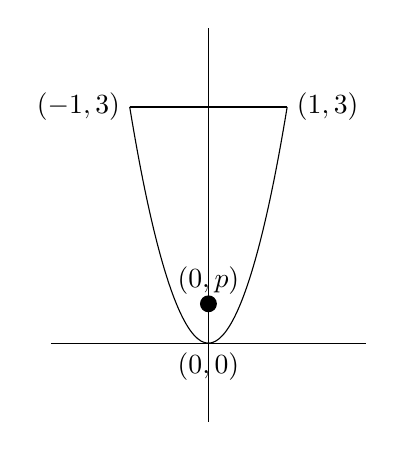
\begin{tikzpicture}
    \draw (-2,0) -- (2,0);
    \draw (0,-1) -- (0,4);
    \draw (0,0) parabola (1,3);
    \draw (0,0) parabola (-1,3);
    \draw (-1,3) -- (1,3);
    \node [right] at (1,3) {$(1,3)$};
    \node [left] at (-1,3) {$(-1,3)$};
    \node [below] at (0,0) {$(0,0)$};
    \draw [fill=black] (0,0.5) circle [radius=0.1];
    \node [above] at (0,0.5) {$(0,p)$};
  \end{tikzpicture}

  \[x^2=4py\]
  \[1^2=4p(3)\]
  \[1=12p\]
  \[p=\frac{1}{12}\]

  So the focus should be located 1/12 ft above the bottom, or 1 inch.

  \bigskip

\item The earth's orbit around the sun is elliptical with the sun at one of
  the foci. The closest the earth gets to the sun is about 91 million miles.
  The eccentricity of the earth's orbit is about 0.0167. What is the farthest
  distance between the earth and the sun?

  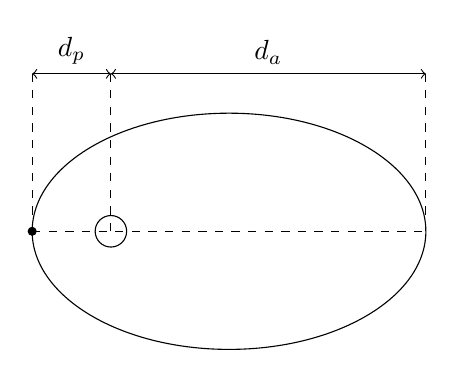
\begin{tikzpicture}
    \draw (0,0) ellipse (2.5 and 1.5);
    \draw [dashed] (-2.5,0) -- (2.5,0);
    \draw (-1.5,0) circle [radius=0.2];
    \draw [fill=black] (-2.5,0) circle [radius=0.05];
    \draw [dashed] (-2.5,0) -- (-2.5,2);
    \draw [dashed] (-1.5,0) -- (-1.5,2);
    \draw [dashed] (2.5,0) -- (2.5,2);
    \draw [<->] (-2.5,2) -- (-1.5,2);
    \draw [<->] (-1.5,2) -- (2.5,2);
    \node [above] at (-2,2) {$d_p$};
    \node [above] at (0.5,2) {$d_a$};
  \end{tikzpicture}

  The closest point is called the \emph{perihelion}; call this distance $d_p$.
  The farthest point is called the \emph{aphelion}; call this distance $d_a$.
  
  We are given:
  \[d_p=a-c=91\ \mbox{million miles}\]
  \[e=\frac{c}{a}=0.0167\]
  Note that:
  \[d_a=2a-(a-c)=a+c\]
  But we can solve for $a$ and $c$:
  \begin{eqnarray*}
    c &=& ae \\
    d_p &=& a-ae \\
    d_p &=& a(1-e) \\
    a &=& \frac{d_p}{1-e} \\
    c &=& d_p\left(\frac{e}{1-e}\right) \\
    d_a &=& \frac{d_p}{1-e}+d_p\left(\frac{e}{1-e}\right) \\
    &=& \frac{d_p+d_pe}{1-e} \\
    &=& d_p\left(\frac{1+e}{1-e}\right) \\    
    &=& 91\left(\frac{1+0.0167}{1-0.0167}\right) \\
    &\approx& 94 \\
  \end{eqnarray*}

  $d_a\approx94$ million miles

  \bigskip

\item Consider the following parabola:
  \[y^2-6y-12x+33=0\]
  \begin{enumerate}
  \item What is the vertex?
    \begin{eqnarray*}
      y^2-6y &=& 12x-33 \\
      y^2-6y+9 &=& 12x-33+9 \\
      (y-3)^2 &=& 12x-24 \\
      (y-3)^2 &=& 12(x-2) \\
    \end{eqnarray*}
    $V(2,3)$
    
  \item What is the axis of symmetry?
    \[y=3\]
    
  \item What is the focus?
    \[4p=12\]
    \[p=3\]
    \[F(2+p,3)=F(5,3)\]
    
  \item What is the directrix?
    \[x=2-p=2-3=-1\]
    
  \item What is the focal diameter?
    \[d=\abs{4p}=4\cdot3=12\]
    
  \item Sketch the parabola, labeling all of the above items.
    
    \begin{tikzpicture}[scale=0.5]
      \draw (-5,0) -- (10,0);
      \draw (0,-5) -- (0,10);
      \draw [domain=2:6] plot({\x},{sqrt(12*(\x-2))+3});
      \draw [domain=2:6] plot({\x},{-sqrt(12*(\x-2))+3});
      \draw [dashed] (-1,-5) -- (-1,10);
      \draw [dashed] (-5,3) -- (10,3);
      \draw [fill=black] (2,3) circle [radius=0.1];
      \draw [fill=black] (5,3) circle [radius=0.1];
      \node [below] at (2,3) {$(2,3)$};
      \node [below] at (5,3) {$(5,3)$};
      \node [below left] at (-1,0) {$-1$};
    \end{tikzpicture}
  \end{enumerate}

\item Consider the following ellipse:
  \[4x^2+25y^2-50y-75=0\]
  \begin{enumerate}
  \item What is the center?
    \begin{eqnarray*}
      4x^2+25(y^2-2y) &=& 75 \\
      4x^2+25(y^2-2y+1) &=& 75+25 \\
      4x^2=25(y-1)^2 &=& 100 \\
      \frac{x^2}{25}+\frac{(y-1)^2}{4} &=& 1 \\
      \frac{x^2}{5^2}+\frac{(y-1)^2}{2^2} &=& 1 \\
    \end{eqnarray*}

    $C(0,1)$
    
  \item What is the length of the major axis?
    \[a=5\]
    \[2a=10\]
    
  \item What is the length of the minor axis?
    \[b=2\]
    \[2b=4\]
    
  \item What are the four vertices?
    \[\begin{array}{l}
      V_1(5,1) \\
      V_2(-5,1) \\
      V_3(0,3) \\
      V_4(0,-1) \\
    \end{array}\]

  \item What are the two foci?
    \[c^2=a^2-b^2=25-4=21\]
    \[c=\sqrt{21}\]
    \[F(\pm\sqrt{21},1)\]

  \item Sketch the ellipse, labeling all of the above items.

    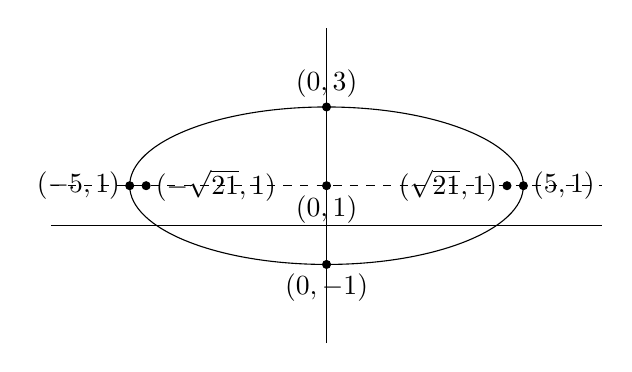
\begin{tikzpicture}[scale=0.5]
      \draw (-7,0) -- (7,0);
      \draw (0,-3) -- (0,5);
      \draw (0,1) ellipse (5 and 2);
      \draw [dashed] (-7,1) -- (7,1);
      \draw [fill=black] (0,1) circle [radius=0.1];
      \draw [fill=black] ({sqrt(21)},1) circle [radius=0.1];
      \draw [fill=black] ({-sqrt(21)},1) circle [radius=0.1];
      \draw [fill=black] (-5,1) circle [radius=0.1];
      \draw [fill=black] (5,1) circle [radius=0.1];
      \draw [fill=black] (0,3) circle [radius=0.1];
      \draw [fill=black] (0,-1) circle [radius=0.1];
      \node [below] at (0,1) {$(0,1)$};
      \node [above] at (0,3) {$(0,3)$};
      \node [below] at (0,-1) {$(0,-1)$};
      \node [right] at (5,1) {$(5,1)$};
      \node [left] at (-5,1) {$(-5,1)$};
      \node [left] at ({sqrt(21)},1) {$(\sqrt{21},1)$};
      \node [right] at ({-sqrt(21)},1) {$(-\sqrt{21},1)$};
    \end{tikzpicture}
  \end{enumerate}

\item Consider the following hyperbola:
  \[36x^2+72x-4y^2+32y+116=0\]
  \begin{enumerate}
  \item What is the center?
    \begin{eqnarray*}
      36(x^2+2x)-4(y^2-8y) &=& -116 \\
      36(x^2+2x+1)-4(y^2-8y+16) &=& -116+36-64 \\
      36(x+1)^2-4(y-4)^2 &=& -144 \\
      \frac{(y-4)^2}{36}-\frac{(x+1)^2}{4} &=& 1 \\
      \frac{(y-4)^2}{6^2}-\frac{(x+1)^2}{2^2} &=& 1 \\
    \end{eqnarray*}

    $C(-1,4)$
    
  \item What is the length of the horizontal axis?
    \[b=2\]
    \[2b=4\]
    
  \item What is the length of the vertical axis?
    \[a=6\]
    \[2a=12\]
    
  \item What are the two vertices?
    \[\begin{array}{l}
    V_1(-1,10) \\
    V_2(-1,-2) \\
    \end{array}\]
    
  \item What are the two foci?
    \[c^2=a^2+b^2=36+4=40\]
    \[c=\sqrt{40}=2\sqrt{10}\]
    \[F(-1,4\pm2\sqrt{10})\]
    
  \item What are the two asymptotes?
    
    \begin{minipage}{2in}
      \[(y-4)=\frac{6}{2}(x+1)\]
      \[y=3x+7\]
    \end{minipage}
    \begin{minipage}{2in}
      \[(y-4)=-\frac{6}{2}(x+1)\]
      \[y=-3x+1\]
    \end{minipage}
    
  \item Sketch the hyperbola, labeling all of the above items.

    \begin{tikzpicture}[scale=0.5]
      \draw (-10,0) -- (10,0);
      \draw (0,-9) -- (0,17);
      \draw [fill=black] (-1,4) circle [radius=0.1];
      \draw [fill=black] (-1,10) circle [radius=0.1];
      \draw [fill=black] (-1,-2) circle [radius=0.1];
      \draw [fill=black] (-1,{4+sqrt(40)}) circle [radius=0.1];
      \draw [fill=black] (-1,{4-sqrt(40)}) circle [radius=0.1];
      \draw [domain=-4.5:2.5] plot({\x},{6*sqrt(1+(\x+1)^2/4)+4});
      \draw [domain=-4.5:2.5] plot({\x},{-6*sqrt(1+(\x+1)^2/4)+4});
      \draw [fill=black] (1,10) circle [radius=0.1];
      \draw [fill=black] (-3,10) circle [radius=0.1];
      \draw [fill=black] (1,-2) circle [radius=0.1];
      \draw [fill=black] (-3,-2) circle [radius=0.1];
      \draw [dashed] (1,10) -- (-3,10) -- (-3,-2) -- (1,-2) -- (1,10);
      \draw [dashed] (-5,-8) -- (3,16);
      \draw [dashed] (-5,16) -- (3,-8);
      \node [right] at (1,10) {$(1,10)$};
      \node [right] at (1,-2) {$(1,-2)$};
      \node [left] at (-3,10) {$(-3,10)$};
      \node [left] at (-3,-2) {$(-3,-2)$};
      \node [right] at (-1,4) {$(-1,4)$};
      \node [below] at (-1,10) {$(-1,10$};
      \node [above] at (-1,-2) {$(-1,-2$};
      \node [above] at (-1,{4+sqrt(40)}) {$(-1,4+2\sqrt{10})$};
      \node [below] at (-1,{4-sqrt(40)}) {$(-1,4-2\sqrt{10})$};
      \node [right] at (3,16) {$y=3x+7$};
      \node [left] at (-5,16) {$y=-3x+1$};
    \end{tikzpicture}
  \end{enumerate}
\end{enumerate}
\end{document}
